%\documentclass[11pt]{article}
\documentclass[10pt,a4paper]{article}
\usepackage[top=30pt,bottom=32pt,left=48pt,right=46pt]{geometry}
%Gummi|065|=)
\title{\textbf{Transcript Abundance Estimation Using Expectation-Maximization Algorithm}}
\author{Mir Imtiaz Mostafiz (0417052041)\\
		S.M.Farabi Mahmud (0417052068)\\
		}
\date{}
\usepackage{multirow}
\usepackage{amsmath}
\usepackage{makecell}
\usepackage{graphicx}
\usepackage{hyperref}
\usepackage{cite}
\begin{document}

\maketitle

\section*{Introduction \& motivation}
\textbf{Transcript Abundance Estimation} is a problem which finds relative abundances of different RNA-transcripts from a set of reads, where the reads themselves were generated from those transcripts.\\
Expectation-Maximization Algorithm is a systematic way to deduce the unknown parameters of a system, from some known observations and some known parameters of a system, through multiple iterations of expectations and maximizations.\\
In this note, a bridge will be constructed between the concepts stated above.

\section*{Prerequisites}
To understand this topic, you need to have some basic knowledge about:
\begin{itemize}
\item \textbf{Basic of Probability and Distributions}: Different kinds of distributions and their mean, variance, likelihood; Sampling, Events.
\item \textbf{Central Dogma of Genetics}: Interactive relations between DNAs, RNAs and Proteins.
\item \textbf{Some Advanced Concepts of Computational Biology}:
\begin{itemize}
    \item Short Read Mapping
    \item Alternative Splicing
    \item *-seq
    \item RNA-seq
\end{itemize}



\end{itemize}

\begin{enumerate}
\item \textbf{Basic of Probability and Distributions}: Different kinds of distributions and their mean, variance, likelihood; Sampling, Events.
\item \textbf{Central Dogma of Genetics}: Interactive relations between DNAs, RNAs and Proteins.
\item \textbf{Some Advanced Concepts of Computational Biology}: Short Read Mapping, Alternative Splicing, *-seq, RNA-seq etc.
\item For absolutely nothing

\begin{enumerate}
    \item Short Read Mapping
    \begin{enumerate}
    \item one
    \item two
    \end{enumerate}
    \item Alternative Splicing
    \item *-seq
    \item RNA-seq
\end{enumerate}
\end{enumerate}


\section{Expectation-Maximization Algorithm}

\subsection{Prelude}
Every system, or experimental setup, consists of three basic parts: system parameters, event observations and unknown quantities( observations/parameters). In ideal and most favorable situations, we usually use the parameters and observations to deduce the unknowns. A such experimental setup , credited to~\cite{do2008expectation}, is described below.\\

Let's assume, there are two coins, $A$ and $B$. The probability that the head side is up after tossing coin $A$ is $\theta_{A}$ (so the probability that the tail side is up after tossing coin $A$ is $1-\theta_{A}$  ). Similarly, the probability that the head side is up after tossing coin $B$ is $\theta_{B}$ (so the probability that the tail side is up after tossing coin $B$ is $1-\theta_{B}$  ). The probability of picking a coin is uniformly distributed, i.e. probability of picking coin A is $P(A)=0.50$ and so is the probability of picking coin B, $P(B)$. To determine $\theta_A$ and $\theta_B$, we will follow this procedure:\\
\begin{itemize}
\item \textbf{Step 1}: Pick a coin (A or B).
\item \textbf{Step 2}: Toss it 10 times and tally the head/tail events.
\item \textbf{Step 3}: Run the steps 1 \& 2 for 5 times.
\item \textbf{Step 4}: Determine $\theta_A$ and $\theta_B$ from the tallied event counts using the law of maximum-log-likelihood.
\end{itemize} 

So, the system can be described like this in table~\ref{exp1} (the observations are shown as an example):\\

% Please add the following required packages to your document preamble:
% \usepackage{multirow}
\begin{table}[h]
\centering
\caption{Experimental Setup (Example)}
\label{exp1}
\begin{tabular}{|l|l|}
\hline
\multirow{2}{*}{Known Parameters}                 & $P(A)=0.5$ \\ \cline{2-2}
                                                  & $P(B)=0.5$ \\ \hline
                                                                  
\multirow{5}{*}{Observed Events} & Coin B: HTTTHHTHTH \\ \cline{2-2} 
                   & Coin A: HHHHTHHHHH \\ \cline{2-2} 
                   & Coin A: HTHHHHHTHH \\ \cline{2-2} 
                   & Coin B: HTHTTTHHTT \\ \cline{2-2} 
                   & Coin A: THHHHHTHTH \\ \hline
Unknown Quantities                  & $\theta_A$ and $\theta_B$ \\ \hline
           
\end{tabular}
\end{table}
\begin{table}[]
\centering
\caption{My caption}
\label{my-label}
\begin{tabular}{|l|l|l|l|l|}
\hline
eee & e          & d         &  &  \\ \hline
    & \multicolumn{2}{l|}{d} &  &  \\ \hline
    &            &           &  &  \\ \hline
    &            &           &  &  \\ \hline
\end{tabular}
\end{table}

We know that the population mean of an observation set sampled from Bernouli distribution is simply their average. From table~\ref{exp1}, the tallies of coin flips can be shown in table~\ref{exp2}.

\begin{table}[]
\centering
\caption{Coin Flip Tallies (Example)}
\label{exp2}

\begin{tabular}{|l|l|l|}
\hline
	Observations & Coin A & Coin B\\
\hline
	HTTTHHTHTH &  & 5H,5T\\
\hline
	HHHHTHHHHH & 9H,1T & \\
\hline
	HTHHHHHTHH & 8H,2T & \\
\hline
	HTHTTTHHTT &  & 4H,6T\\
\hline
	THHHHHTHTH & 7H,3T & \\
\hline
	Total & 24H,6T & 9H,11T\\
\hline
\end{tabular}
\end{table}
So, as per \textbf{Maximum Likelihood Estimation (MLE)} rules, ${\theta_{A}}^{\prime}=\frac{\text{Heads from A}}{\text{Heads from A + Tails from A}}=\frac{24}{24+6}=0.8$ and ${\theta_{B}}^{\prime}=\frac{\text{Heads from B}}{\text{Heads from B + Tails from B}}=\frac{9}{9+11}=0.45$.\\
So, given the parameters and observations of a system, we could deduce some of the unknown parameters using MLE. But what, if, some of the necessary parameters, or some of the necessary observation details( like from which coins the observations were generated) are missing? \textbf{Expectation-Maximization Algorithm} is the answer.

\subsection{Expectation Maximization Algorithm Explanation}

To explain \textbf{Expectation Maximization Algorithm} (EM), we will manipulate the experimental setup described previously. We will assume that the information about which coins were tossed when will not be present.\\
At first, let's brief the basic steps of EM in short:
\begin{itemize}
\item Step 1: Assume the unknown parameters.
\item Step 2: Using the current parameters, both known and hidden (assumed), deduce the expected value of different quantities needed for unknown parameter computation.
\item Step 3: Compute the new values of unknown parameters.
\item Step 4: Repeat steps 2 \& 3 until convergence.

\end{itemize} 

Now, we will explain this process using the converted example. Table~\ref{exp3} shows the current setup, without mentioning the origin of observations (which coins generated which tosses). As we have to determine the value of unknown parameters $\theta_A$ and $\theta_B$, we will assume some values of them, i.e. ${\theta_A}^{(0)}=0.60$ and ${\theta_B}^{(0)}=0.50$ initially. Also, as the origins are not mentioned, we cannot compute the heads and tails in each sets of observations straightforward. Rather, we need to compute the expected number of heads and tells for each type of coins. This expected value calculation is explained below:\\

Let $n$ tosses of coin $X$ generated events $x_1,x_2, \ldots, x_n$, where each $x_i \in \{H,T\}$ and $X \in \{A,B\}$. The posterior probability of $X$ being A can be calculated from priors and likelihoods as, 
\[ P(A \rvert x_1,x_2, \ldots, x_n )= \frac{P( x_1,x_2, \ldots, x_n  \rvert A)P(A)}{P(x_1,x_2, \ldots, x_n )}\] \[\implies P(A \rvert x_1,x_2, \ldots, x_n )= \frac{P( x_1\rvert A)P(x_2 \rvert A)\ldots P(x_n \rvert A)P(A)}{P(x_1,x_2, \ldots, x_n )} \\\tag*{[Because the coin tosses are independent]}\]
Similarly, \[P(B \rvert x_1,x_2, \ldots, x_n )= \frac{P( x_1\rvert B)P(x_2 \rvert B)\ldots P(x_n \rvert B)P(B)}{P(x_1,x_2, \ldots, x_n )}\].

Combining and dividing both equations, we get new equation,
\[ \frac{ P(A \rvert x_1,x_2, \ldots, x_n )}{ P(B \rvert x_1,x_2, \ldots, x_n )} = \frac{P( x_1\rvert A)P(x_2 \rvert A)\ldots P(x_n \rvert A)P(A)}{P( x_1\rvert B)P(x_2 \rvert B)\ldots P(x_n \rvert B)P(B)}\]\[ \implies 
\frac{ P(A \rvert x_1,x_2, \ldots, x_n )}{ P(B \rvert x_1,x_2, \ldots, x_n )} = \frac{P( x_1\rvert A)P(x_2 \rvert A)\ldots P(x_n \rvert A)}{P( x_1\rvert B)P(x_2 \rvert B)\ldots P(x_n \rvert B)} \\\tag*{[Because $P(A)=P(B)=0.5$]}
\]\\
If $x_i= H$, then $P(x_i \rvert A)= \theta_{A}$ and if $x_i= T$, then $P(x_i \rvert A)=1- \theta_{A}$. Similarly, if $x_i= H$, then $P(x_i \rvert B)= \theta_{B}$ and if $x_i= T$, then $P(x_i \rvert B)=1- \theta_{B}$.\\
If there are $k$ heads, then there will be $n-k$ tails, and the equation will look like,
\[ \frac{ P(A \rvert x_1,x_2, \ldots, x_n )}{ P(B \rvert x_1,x_2, \ldots, x_n )} = \frac{ {\theta_{A}}^{k}{(1-\theta_{A})}^{n-k} }{ {\theta_{B}}^{k}{(1-\theta_{B})}^{n-k}}\]
\[\implies 
\frac{ P(A \rvert x_1,x_2, \ldots, x_n )}{P(A \rvert x_1,x_2, \ldots, x_n )+ P(B \rvert x_1,x_2, \ldots, x_n )} = \frac{{\theta_{A}}^{k}{(1-\theta_{A})}^{n-k}}{{\theta_{A}}^{k}{(1-\theta_{A})}^{n-k}+ {\theta_{B}}^{k}{(1-\theta_{B})}^{n-k}}
\]
\[\implies 
P(A \rvert x_1,x_2, \ldots, x_n ) = \frac{{\theta_{A}}^{k}{(1-\theta_{A})}^{n-k}}{{\theta_{A}}^{k}{(1-\theta_{A})}^{n-k}+ {\theta_{B}}^{k}{(1-\theta_{B})}^{n-k}}
\]Similarly, \[P(B \rvert x_1,x_2, \ldots, x_n ) = \frac{{\theta_{B}}^{k}{(1-\theta_{B})}^{n-k}}{{\theta_{A}}^{k}{(1-\theta_{A})}^{n-k}+ {\theta_{B}}^{k}{(1-\theta_{B})}^{n-k}}
\].

\begin{table}[]
\centering
\caption{Experimental Setup 2 (Example)}
\label{exp3}
\begin{tabular}{|l|l|}
\hline
\multirow{2}{*}{Known Parameters}                 & $P(A)=0.5$ \\ \cline{2-2}
                                                  & $P(B)=0.5$ \\ \hline
                                                                  
\multirow{5}{*}{Observed Events} & HTTTHHTHTH \\ \cline{2-2} 
                   & HHHHTHHHHH \\ \cline{2-2} 
                   & HTHHHHHTHH \\ \cline{2-2} 
                   & HTHTTTHHTT \\ \cline{2-2} 
                   & THHHHHTHTH \\ \hline

Unknown Quantities                  & $\theta_A$ and $\theta_B$ \\ \hline
Assumed Quantities                  & ${\theta_A}^{(0)}=0.60$ and ${\theta_B}^{(0)}=0.50$ \\ \hline
           
\end{tabular}
\end{table}


Now, the expected number of $H$ and $T$ from $\{x_1,x_2, \ldots, x_n\}$ from type $A$ if there are $k$ $H$'s and $n-k$ $T$'s are respectively,
\[{\lvert  H \rvert}_{expected}^{A} = \text{Probability that the observations are from A} \times \text{number of H} \] 
\[\implies {\lvert  H \rvert}_{expected}^{A} = P(A \rvert x_1,x_2, \ldots, x_n ) \times k \]
\[\implies 
 {\lvert  H \rvert}_{expected}^{A}= \frac{{ {\theta_{A}}^{(0)}}^{k}{(1-{\theta_{A}}^{(0)} ) }^{n-k}}{{{{\theta_{A}}^{(0)}}^{k}}{(1-{\theta_{A}}^{(0)})}^{n-k}+ {{\theta_{B}}^{(0)}}^{k}{(1-{\theta_{B}}^{(0)})}^{n-k}} \times k
\]
For first set of observations,
\[\implies {\lvert  H \rvert}_{expected}^{A^{(1)}} = \frac{ {(0.6)}^{5} {(1-0.6)}^{10-5} } { {(0.6)}^{5}{(1-0.6)}^{10-5} + {(0.5)}^{5}{(1-0.5)}^{10-5}} \times 5 \]
\[\implies {\lvert  H \rvert}_{expected}^{A^{(1)}} = 0.45 * 5 =2.25\]

Similarly, for first observations, we can deduce,
\[{\lvert  T \rvert}_{expected}^{A^{(1)}} = 0.45 * 5 =2.25\]
\[{\lvert  H \rvert}_{expected}^{B^{(1)}} = 0.55 * 5 =2.75\]
\[{\lvert  T \rvert}_{expected}^{B^{(1)}} = 0.55 * 5 =2.75\]


 


For each set of observations, we deduce this quantities and calculate the estimated MLE from table~\ref{exp4},\\
\begin{table}[h]
\centering
\caption{MLE Computation (Example)}
\label{exp4}
\begin{tabular}{|l|l|l|}
\hline
            
Observations & Coin A & Coin B \\ \hline                                                      
HTTTHHTHTH & 2.25 H, 2.25 T & 2.75 H, 2.75 T \\ \hline 
        HHHHTHHHHH & 7.2 H, 0.8 T& 1.8 H, 0.2 t\\ \hline 
                    HTHHHHHTHH & 5.9 H, 1.5 
T &  
2.1 H, 0.5 
T\\ \hline 
                    HTHTTTHHTT & 1.4 H, 2.1 T & 2.6 H, 3.9 T\\ \hline 
                    THHHHHTHTH & 4.5 H, 1.9 
T & 2.5 H, 1.1 T\\ \hline
Total & 21.3 H, 8.6 T & 11.7H, 8.4 T \\ \hline
                       
\end{tabular}
\end{table}


\[{\theta_{A}}^{(1)} =\frac{{\lvert  H \rvert}_{expected}^{A^{(total)}}}{{\lvert  H \rvert}_{expected}^{A^{(total)}}+{\lvert  T \rvert}_{expected}^{A^{(total)}}} = \frac{21.3}{21.3+8.6}=0.71\]
\[{\theta_{B}}^{(1)} = \frac{{\lvert  H \rvert}_{expected}^{B^{(total)}}}{{\lvert  H \rvert}_{expected}^{B^{(total)}}+{\lvert  T \rvert}_{expected}^{B^{(total)}}} =  \frac{11.7}{11.7+8.4}=0.58\]
 So, starting with assuming values $0.60$ and $0.50$, we ended with $0.71$ and $0.58$ after first iteration. The values will converge after some iterations to $0.80$ and $0.52$ respectively.
 
The step where we calculated the expected numbers of heads and tails is called the \textbf{Expectation} step. The step where we calculated the new estimated value of MLE is known as the \textbf{maximization} step. We repeat these two steps one after another in EM algorithm. 
 
We can summarize the uses and steps of EM algorithm in table~\ref{exp5}.

\begin{table}[h]
\centering
\caption{When's and how's of EM}
\label{exp5}

\begin{tabular}{|l|l|}
\hline
	\thead{When to apply} & \thead{How to apply} \\
\hline
	\makecell{Some parts of the data\\ is hidden} & \makecell{Initially guess the parameters\\ of the model}
 \\
\hline
	\makecell{If we know the parameters\\ to be estimated,\\ we can calculate\\ probabilities of the hidden variables} 
 & \makecell{\textbf{Expectation (E) step} : Use current parameters\\ (and observations)\\ to reconstruct the hidden structure}
 \\
\hline
	\makecell{If we know the values\\ of hidden variables,\\ we can estimate the parameters} & \makecell{\textbf{Maximization (M) step} :\\ Use that hidden structure  \\(and observations)\\ to re-estimate parameters}
 \\
\hline
\end{tabular}
\end{table} 


\section{Transcript Abundance Estimation}
Before getting a detailed view about \textbf{Transcript Abundance Estimation (TAE)}, we will revisit the \textit{Central Dogma} of genetics: a workflow assumption based on which the whole genetics is based.
\subsection{Central Dogma}
Statement: \textit{\textbf{Instructions on DNA are transcribed onto messenger RNA. Ribosomes are able to read the genetic information inscribed on a strand of messenger RNA and use this information to string amino acids together into a protein.}}~\cite{cdogma2017}.\\
Explanation: The central dogma of molecular biology describes the flow of genetic information in cells from DNA to messenger RNA (mRNA) to protein.  It states that genes specify the sequence of mRNA molecules, which in turn specify the sequence of proteins. In technical terms, the central dogma consists of two steps:\\
\begin{description}
\item [Transcription] The information stored in DNA is so central to cellular function, the cell keeps the DNA protected and copies it in the form of RNA. An enzyme adds one nucleotide to the mRNA strand for every nucleotide it reads in the DNA strand~\cite{cdogma2017}.
\item [Translation]  The translation of information to a protein is more complex because three mRNA nucleotides correspond to one amino acid in the polypeptide sequence~\cite{cdogma2017}.

\begin{figure}[htp]
\centering
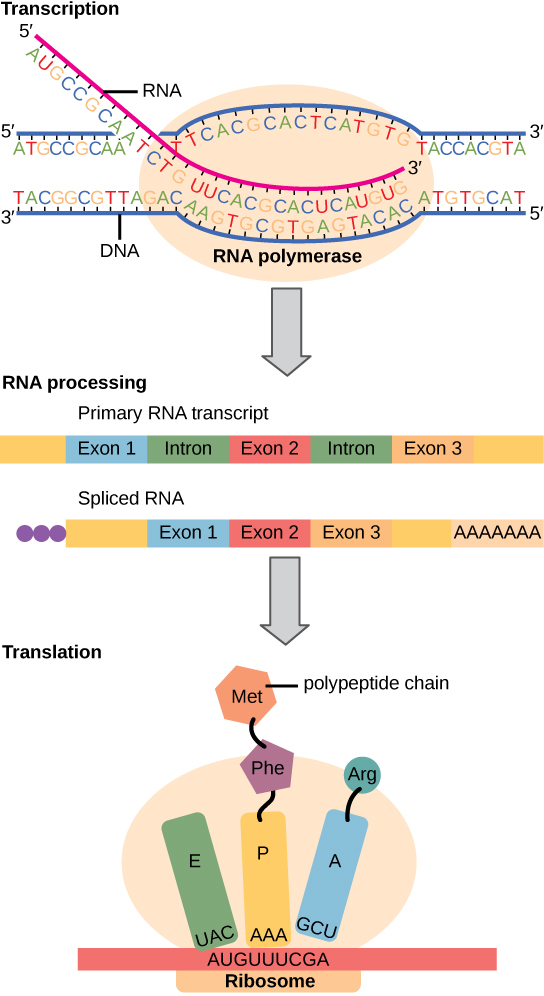
\includegraphics[scale=1.00]{centraldogma.jpeg}
\caption{Central Dogma~\cite{cdogma2017}}
\label{cdog}
\end{figure}
\end{description}

\subsection{Some related terms to know}

\subsubsection{DNA sequencing}
DNA sequencing is the process of determining the precise order of nucleotides within a DNA molecule. It includes any method or technology that is used to determine the order of the four bases—adenine, guanine, cytosine, and thymine—in a strand of DNA~\cite{wiki:dnaseq}. 

\begin{figure}[htp]
\centering
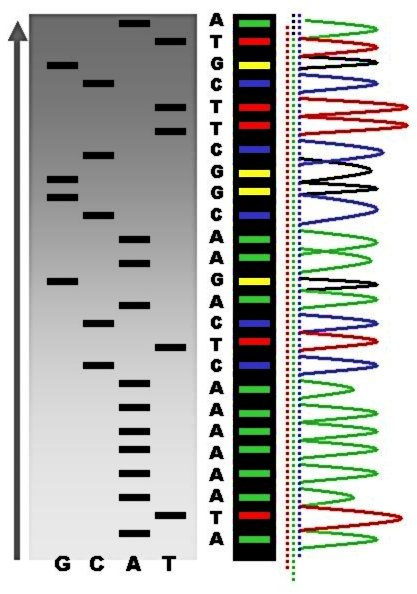
\includegraphics[scale=0.50]{Radioactive_Fluorescent_Seq.jpg}
\caption{An example of the results of automated chain-termination DNA sequencing~\cite{wiki:dnaseq}.}
\label{seq}
\end{figure}
\subsubsection{Transcript}

A primary transcript is the single-stranded ribonucleic acid (RNA) product synthesized by transcription of DNA, and processed to yield various mature RNA products such as mRNAs, tRNAs, and rRNAs. The primary transcripts designated to be mRNAs are modified in preparation for translation. For example, a precursor messenger RNA (pre-mRNA) is a type of primary transcript that becomes a messenger RNA (mRNA) after processing~\cite{wiki:pritrans}.

\subsubsection{Alternative Splicing}
Alternative splicing, or differential splicing, is a regulated process during gene expression that results in a single gene coding for multiple proteins. In this process, particular exons of a gene may be included within or excluded from the final, processed messenger RNA (mRNA) produced from that gene~\cite{ wiki:altsp} (see fig~\ref{iso}).

\subsubsection{Protein Isoform}

A protein isoform, or "protein variant"[1] is a member of a set of highly similar proteins that perform the same or similar biological roles. A set of protein isoforms may be formed from alternative splicings or other post-translational modifications of a single gene~\cite{wiki:proiso} (see figure~\ref{iso}). \begin{figure}[htp]
\centering
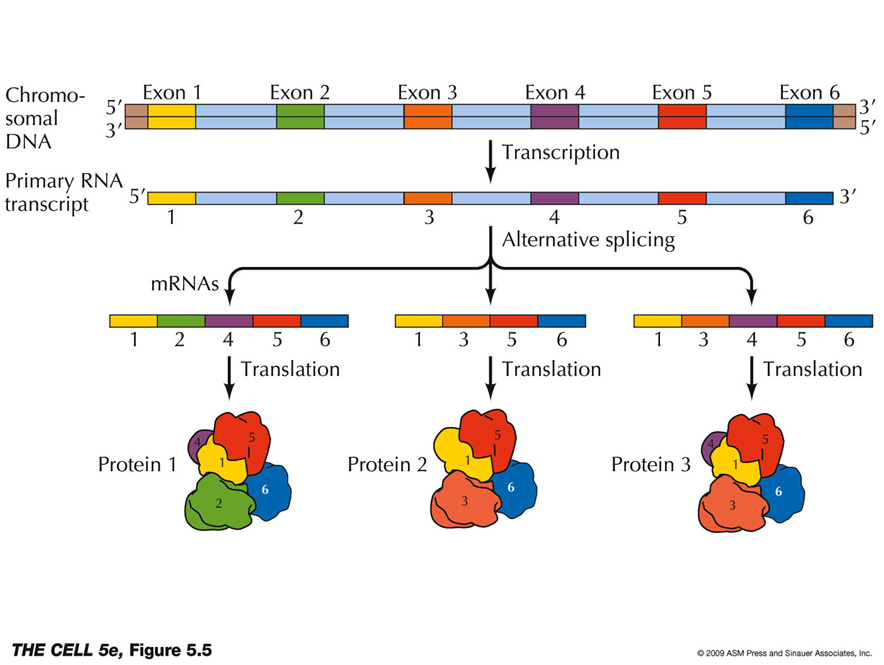
\includegraphics[scale=0.50]{proiso.png}
\caption{Protein A, B and C are isoforms encoded from the same gene through alternative splicing~\cite{wiki:altsp}}
\label{iso}
\end{figure}
\subsubsection{Short Read Alignment}

Short read alignment is the process of figuring out where in the genome a sequence is from. By transcription process we get the mRNAs from DNA. By putting them through a reverse transcription and sequencing pipeline, we can get the sequences corresponding to the RNA transcript. A huge task after this is finding the place in the genome from where that gene sequence generated. This is done by short read alignment algorithms.

\subsubsection{*-seq}
*-seq is a generalized term used to denote the class of high-throughput selection algorithms. The full list of *-seq algorithms can be found at \url{https://liorpachter.wordpress.com/seq/}.

\subsubsection{RNA-seq}
RNA-Seq (RNA sequencing), also called whole transcriptome shotgun sequencing  (WTSS), uses next-generation sequencing (NGS) to reveal the presence and quantity of RNA in a biological sample at a given moment in time. The process of RNA-seq has been described in~\cite{wiki:rnaseq} (see figure~\ref{rnaseq}.

\begin{figure}[htp]
\centering
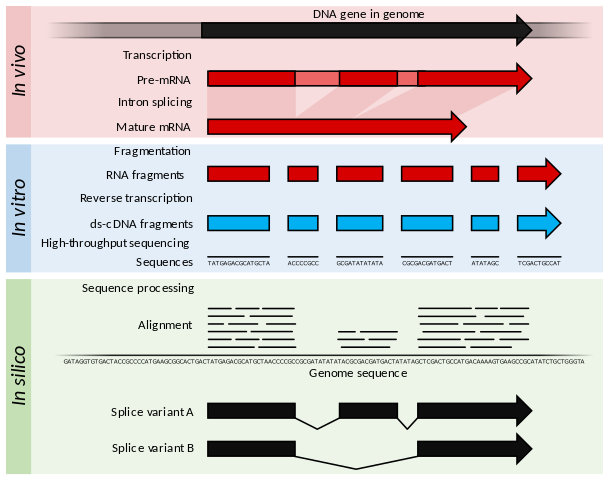
\includegraphics[scale=0.70]{Summary_of_RNA-Seq.svg.png}
\caption{Summary of RNA-Seq. Within the organisms, genes are transcribed and spliced (in eukaryotes) to produce mature mRNA transcripts (red). The mRNA is extracted from the organism, fragmented and copied into stable ds-cDNA(blue). The ds-cDNA is sequenced using high-throughput, short-read sequencing methods. These sequences can then be aligned to a reference genome sequence to reconstruct which genome regions were being transcribed. This data can be used to annotate where expressed genes are, their relative expression levels, and any alternative splice variants~\cite{wiki:rnaseq}.}
\label{rnaseq}
\end{figure} 

\subsection{Relative Transcript Abundance Estimation}

Sequencing RNAs are easier than sequencing proteins. In genetics, there might often be the necessity of knowing the proportion of proteins present in a cell. However, as protein sequencing is replaced by RNA-sequencing as a proxy, we are interested in finding the \textit{Relative Transcript Abundance} of the RNA-transcripts: which deals with the percentage amount of the RNA-transcripts present in a set of cell or genome reads.\\ 

\subsubsection{Challenges and motivation}
Usually, in theoritical term, to compute the relative abundances, it is obvious to count the amount of reads from a transcript and deduce the parameters thereby. But there are some challenges. Due to the presence of isoform, it can happen that a single sequence read may be mapped to multiple transcripts while short read mapping. This multiple mapping pushes us to use the expected number of reads from each transcripts rather than using their exact numbers (remember using the expected number of heads and tails from coins A \& B instead of using the exact counts because we did not know which coins were tossed?).\\
But to use expected value, we need to know the relative abundance of the transcripts again. This poses a deadlock like situation as the coin bias problem stated in previous section, where to know the biases of the coins, we needed to know the expected numbers of heads and tails from different coins, which in turn needed to use coin biases. We solved that problem using EM algorithm. This abundance estimation problem won't be the exception too.\\


In the next section, we will discuss a mathematical model of relative abundance estimation and try to solve it using EM algorithm.
\section{How to use EM Algorithm to solve Transcript Abundance Estimation}
The proof is credited to \cite{pachter2011models}.\\
Let $T$ be the set of transcripts from a RNA-sequencing samples and let $l_t$ be the length of transcript $t \in T$.\\
We define $\rho = \{\rho_t\}_{t \in T}$ be the relative abundances of transcripts such that $\sum_{t \in T}{\rho_t}=1$\\
Let $F$ be the set of reads and $F_t$ be the set of short reads from transcript $t \in T$ ($F_t \subseteq F$).\\
 Let there are $\lvert F \rvert$ reads of length $m$ on average. So, for a transcript $t \in T$, a read could start from $l_t-m+1$ possible locations. This will be denoted as the \textit{effective length} of transcript $t$, $\tilde{l_t}= l_t-m+1$.\\

\subsection{Expectation step} 
As per generative model assumptions, the probability of choosing a transcript $t$ for read is,
\begin{displaymath}
\frac{ {\rho_t}{\tilde{l_t}}  }{ \sum_{r \in T}{ {\rho_r}{\tilde{l_r}}} }
\end{displaymath}

There are $\tilde{l_t}$ possible places for a read from $t$ to start at. So the probability that a read was chosen from transcript $t$ is equal to the product of the probabilities of choosing $t$ and choosing a place from $t$ to start at,
\begin{displaymath}
\frac{ {\rho_t} {\tilde{l_t}}  }{ \sum_{r \in T} { {\rho_r}{\tilde{l_r}}} }
\times \frac{1}{\tilde{l_t}}
\end{displaymath}    

So, we will start the estimation process by assuming some initial values of hidden variables $\rho$.
\subsection{Maximization step}

So, for the set of reads from $t$, the number of reads is $X_t= \lvert F_t \rvert$.\\
To compute the likelihood of the parameter settings $\rho$, we need to compute the probabilities of $f \in F_t$ being generated from transcript $t$,
\begin{displaymath}
{({\frac{ {\rho_t} {\tilde{l_t}}  }{ \sum_{r \in T} { {\rho_r}{\tilde{l_r}}} }
\times \frac{1}{\tilde{l_t}}
})}^{X_t}
\end{displaymath}

So, the likelihood for parameter settings $\rho$ is,

\begin{displaymath} {\mathbf{L}(\rho)}=\prod_{t \in T}{{({\frac{ {\rho_t} {\tilde{l_t}}  }{ \sum_{r \in T} { {\rho_r}{\tilde{l_r}}} }
\times \frac{1}{\tilde{l_t}}
})}^{X_t}}
\end{displaymath}

Let, $\alpha_t=\frac{ {\rho_t} {\tilde{l_t}}  }{ \sum_{r \in T} { {\rho_r}{\tilde{l_r}}} }
$.\\So,
\begin{displaymath} {\mathbf{L}(\rho)}=\prod_{t \in T}{({\frac{\alpha_t}{\tilde{l_t}}) } ^{X_t} }
\end{displaymath} 
After applying log-likelihood and taking derivatives to find the maxima, we get,
\begin{displaymath}
\hat{\alpha_t}= \frac{{X_t}}{\sum_{t \in T}{{X_t}}}
\end{displaymath},

As ${\sum_{r \in T} { {\rho_r}{\tilde{l_r}}}}$ will be equal for each $t \in T$, we can write,
\begin{displaymath}
\hat{\alpha_t} \propto {{\hat{{\rho_t}} { \tilde{l_t} } } }
\implies  \hat{\rho_t} \propto {{\frac{\hat{\alpha_t}}{\tilde{l_t}}}}
\end{displaymath}
From this calculation, we can re-estimate the value of $\rho$ and use it in next iteration of EM until convergence.

\begin{figure}[h]
\centering
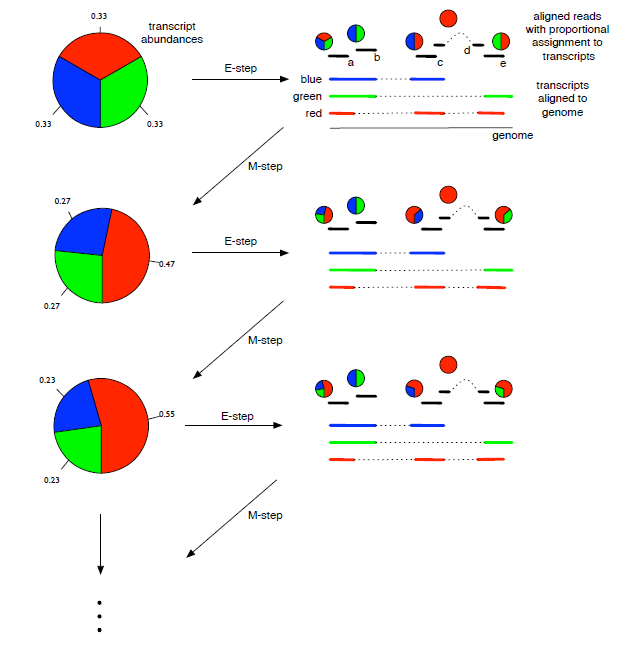
\includegraphics[scale=0.60]{ex.png}
\caption{EM in Transcription Abundance Estimation~\cite{pachter2011models}}
\label{}
\end{figure}

\section{Some related works}
~\cite{li2011rsem} and ~\cite{li2009rna} are two notable works regarding abundance estimation problem.

\bibliography{ref}
\bibliographystyle{acm}
\end{document}
